\documentclass[a4paper,titlepage]{article}

\usepackage[utf8]{inputenc}

\usepackage[
  citestyle=ieee,
  style=ieee]{biblatex}
\addbibresource{bibliography.bib}

\usepackage{fancyhdr}
\pagestyle{fancy}
\fancyhf{}
\rhead{COMP2043.GRP Interim Group Report}
\lhead{Team02}

\usepackage{enumitem}
\setlist[enumerate]{label*=\arabic*.}

\usepackage{graphicx}
\graphicspath{ {./images/} }

\usepackage{alltt, float, multicol}

\begin{document}

\begin{titlepage}
  \centering
  \large{\textsc{COMP2043.GRP Interim Group Report}}\\
  \vspace{3cm}
  \huge{Team02}\\
  \Huge{Machine Learning Dataset Parsing Tool}\\
  \vspace{3cm}
  \LARGE{\textsc{Group Members}}\\
  \Large{Boyuan Ma - zy22053 (Team Leader)}\\
  \Large{Xinyan Li - zy22043}\\
  \Large{Hao Liu - zy22046}\\
  \Large{Xinjie Pang - zy22055}\\
  \Large{Marios Igkiempor - scymi1}\\
  \vspace{1cm}
  \LARGE{\textsc{Supervisor}}\\
  \Large{Chris Roadknight}\\
  \vfill
  \large{\textsc{December 2018}}

\end{titlepage}

\tableofcontents
\pagebreak

\section{Description of the Problem}
Team02's project is centered around a system that classifies datasets by the best type of machine learning approach to take in order to best analyse the data.
It is proposed that the system will be able to parse a dataset, analyse its features and propose a type of machine learning (supervised, semi-supervised and unsupervised), as well as a more specific algorithm, that can best model the dataset based on the analysed features.

The client intends to use the project as both a prefilter for machine learning and as a teaching aid, and so the program should be able to provide useful information as to how the machine learning approach was derived.
However, it should be noted that being an expert in the field, the client expects his knowledge to be captured in the system.
As such, any useful information provided by the system would be used to aid the teaching of students and should therefore be suitable for someone that is not an expert in the field.

Datasets that the program will analyse will be provided by the client, however the system should be able to parse and analyse newly uploaded datasets with the same level of accuracy.

\section{Background Information and \\Relevant Research}

\subsection{Similar Tools}
Although there exist many platforms and libraries for performing machine learning, there does not appear to be any tools to help a user choose the appropriate machine learning methods.
A lot of libraries discovered are implementations of machine learning algorithms, for example \verb|scikit-learn| \cite{scikit-learn} and \verb|Pandas| \cite{pandas} for Python.
There also exist platforms for performing machine learning, such as Weka \cite{weka} and H2o \cite{h2o.ai}.
Although all of these tools are useful for actually performing machine learning, they do not provide the user with any indication as to which machine learning method to use.
They simply abstract the details of each machine learning method.
Given this research, the project seems to be the only one of its kind.

\subsection{Understanding Machine Learning Algorithms}
Section \ref{pickingML} lists the machine learning algorithms that the system will be able to produce as output.
The team felt it would be beneficial to have a basic understanding of each algorithm, their respective principles, and how and when to use each one..
Some background research was conducted into each algorithm.

\subsubsection*{Self-Organising Map}
A Self-Organising Map (SOM) converts complex relationships within data of high dimensions into simple relationships in lower dimensions, all while preserving the most important relationships of the starting data \cite{kohonen2005}.
\subsubsection*{K-Means Clustering}
K-means clustering classifies a set of data into $k$ clusters (where $k > 0$) by assigning it to a centroid (central location of a cluster).
This is achieved by assigning it to the nearest centroid.
When each data point has been assigned, $k$ centroids are recalculated and the datapoints are reassigned.
This process of defining and assigning to new centroids is repeated until no data points move \cite{kmeans}.
\subsubsection*{Principal Component Analysis}
Principal Component Analysis (PCA) finds a small subset of combinations of correlated parameters which have the most influence on variation within the dataset \cite{einasto2011}.
% The data is mapped on a new coordinate systen, where the first axis indicates the component which contributes the most to variance (the principal component), the second axis indicates the second most influencial, and this pattern continues for all parameters.
\subsubsection*{Linear Regression}
Linear Regression is a form of predictive analysis where the values of an independent variable are used to predict future values of a dependent variable by fitting a line through the values of two or more variables \cite{davison2003}.
\subsubsection*{Neural Network}
% Artificial Neural Network (ANN) is a machine learning method simulating information processing of a human brain to build a mathematic model.
% The model consists of processing elements (neurons), each of which have an activation function.
% ANNs require a large amount of examples as training data and test data to complete the model, like the process of human learning.
% It has advantages in processing amounts of fuzzy nonlinear data.
Artificial Neural Networks are networks of processing nodes, each connected via a weight.
The weighted sum of all input values into a node is ran through an activation function.
If the function outputs a number higher than a threshold, its weighted sum is propagated into the input of all nodes connected to its output \cite{hardesty2017}.
\subsubsection*{Multiclass Neural Network}
A Multiclass Neural Network extends on a neural network by providing one output neuron for each possible output class of a given problem \cite{multiclassnn}.
\subsubsection*{Random Forest Regression}
% It performs many times of sampling back to the original data set, and each time extracts the same number of observations as the sample size. Since it is put back into the sample, some observations are not drawn each time, and some observations are repeatedly drawn. You get a lot of different data sets and then build a decision tree for each data set, thus generating a large number of decision trees.
Random Forests select a random subset of features, observe their outputs, and generate a decision tree based on the features selected.
This process is repeates lots of times (hundreds to thousands), and each tree is averaged into the final decision tree. \cite{hastie2017}
\subsubsection*{Logistic Regression}
Logistic Regression is a method for binary prediction when the outputs are dichotomous (true or false).
It is used to find the relationship of one dichotomous variable, and one or more other independent variable. \cite{logisticregression}
\subsubsection*{Multiclass Logistic Regression}
A generalisation of Logistic Regression, which can identify more than two possible outcomes. \cite{greene2012}
\subsubsection*{Naïve Bayesian Network}
% Naïve Bayes is a sorting technique based on Bayes’ theorem.
% It sets characteristics of data as tags and assume that the tags are mutually independent on probability.
% Then the Naïve Bayes Classifier sort the objects and calculates probability according to these tags.
% And the objects can be sorted to known classes or demonstrate the probability of an object belonging to a class.
A Naïve Bayesian Network calculates the conditional probability of each attribute of a class given its label.
By applying Bayes rule, labels are classified based on the instances of each attribute.
Its naïvety stems from the fact that it assumes that all attributes are conditionally independent on the class. \cite{friedman1997bayesian}
\subsubsection*{Support Vector Machine}
% Support Vector Machine (SVM) is a method used to sort and regress.
% SVM is a development of binary liner classifier.
% For the nonlinearities, SVM transforms the sample into higher dimensions so that the sample can be linerly analyzed because of high dimensional features.
Support Vector Machines take an input vector and map it, non-linearly, into a higher dimension feature space, in which a linear decision surface is created.
The decision surface ensures high generalisability. \cite{cortes1995support}
\subsubsection*{Self-Training}
Self training trains a model with labeled data, which is used to classify unlabeled data.
The unlabeled data that the model classified with the highest confidence are added back to the set of labeled data \cite{fazakis2016}.
% \subsubsection*{Forced Clustering}
\subsubsection*{Anti-Learning}
% Anti-learning is used when the accuracy of a trained model's output is worse than random outputs even if no overfitting or over training occurred.
Anti-learning is the situation where a trained model is outperformed by randomly guessing, in the absence overfitting or overtraining \cite{roadknight2015antilearning}.

\section{Requirements Specification}
Following meeting with the client and discussing initial user requirements and system requirements specification, as well as subsequent meeting revising both requirements, the team and the client have agreed on a set of requirements.

\subsection{User Requirements}

\begin{enumerate}
  \item Parse datasets and suggests the best machine learning approaches for modeling that dataset.

  \item The user will supply datasets to be analysed.

  \item The system will need to be appropriate for use as both a prefilter for machine learning and as a teaching aid.

  \item The user requires a degree of data visualization in the front end.

  \item The user requires a comprehensive, extendible database. The database should allow the user to:
  \begin{enumerate}
    \item upload datasets
    \item provide relevant information about the datasets
  \end{enumerate}

  \item A rule-based approach will initially be sufficient to assertain what the ideal machine learning approach is for each dataset.
  The user should be able to affect the decisions made by the rule based system by providing additional information on the structure and complexity of the data.

  \item The system should be deterministic rather than probabilistic, meaning that it provides a machine learning method that it is sure is the best, as opposed to a percentage chance that the method could be the best.
  The same datasets should always map to the same machine learning method.

  \item The client has significant knowledge of machine learning methods and some of this knowledge will need to be captured to facilitate the decision making process.
\end{enumerate}

\subsection{Functional System Requirements}

\begin{enumerate}
  \item The system will require a database which can store the data in every dataset

  \begin{enumerate}
    \item The user can upload the dataset.

    \item The datasets are available for users to download.

    \item Information about the dataset (what type of data, whether or not there are missing values) can be provided by the user and stored as metadata with each dataset.

    \item The datasets need preprocessing to find details about the data. These details must be stored as metadata with the dataset.
    Details will be characteristics of the datasets which help decide the best machine learning approach.
    Such details could include:
    \begin{enumerate}
      \item The type of data
      \item Size of the dataset
      \item Number of features
      \item Number of target outputs provided with the data
      \item Whether or not there are missing values
      \item Whether the labels are categories or values
      \item Complexity of the dataset
      \item Complexity of relations in the dataset
      \item Wether or not the dataset is structured
    \end{enumerate}

    \item The customer needs to be able to add and delete information stored in the database.

    \item The original data must never be altered.
    Any pre-processing or analysis may be available to the user, but the user must also have access to the original data they provided.
  \end{enumerate}

  \item The system must be able to analyze a dataset and provide the best machine learning approach to model the dataset.
  \begin{enumerate}
    \item The reason why that approach is best needs to be provided to the user.

    \item The system will have different cataglogues of machine learning.
    Each cataglogue provides the algorithm for the machine learning and the sample datasets.

    \item The system must have a search engine which can search for both the datasets' name and machine learning approaches.
  \end{enumerate}

  \item The system must provide different types of data visualization
  \begin{enumerate}
    \item Bar charts
    \item Scatter graphs
    \item Images
    \item Interactive visualization at the result page
  \end{enumerate}

  \item The system should have different mapping opinions for finding the ideal machine learning method:
  \begin{enumerate}
    \item Rule-based system
    \item Deterministic mode
    \item Probabilistic mode
  \end{enumerate}

  \item As a long-term goal, the system could actually model the data using the decided machine learning tool and provide a visual output of the model for the user.
\end{enumerate}

\subsection{Non-Functional System Requirements}
\begin{enumerate}
  \item Accessibility
  \begin{enumerate}
    \item The user should be able to upload data using multiple types of input, for example both the mouse and the keyboard.
    \item The system should be accessible on multiple different platforms.
  \end{enumerate}

  \item Data integrity

  The original uploaded data should never be changed. If there are mechanisms in place which change the data, these should not affect the original data

 \item Data Retention

  Data stored on the sever should only be kept there for 30 days as a limit.

  \item Extensibility

  The system should be able to cope with data of no more than 200MB.

 \item Performance:

  The system should be able to analyse new data sets in no longer than 1 minute.

  \item Privacy and Security:

  Data uploaded by a user must have the option to be kept private to the user who uploaded it.
\end{enumerate}

\subsection{Modelling Requirements}
Following the elicitation of user and system requirements, the team decided it was useful to model both.
A simple use case diagram was created first, shown in figure \ref{usecase}.

\begin{figure}[h!]
  \centering
  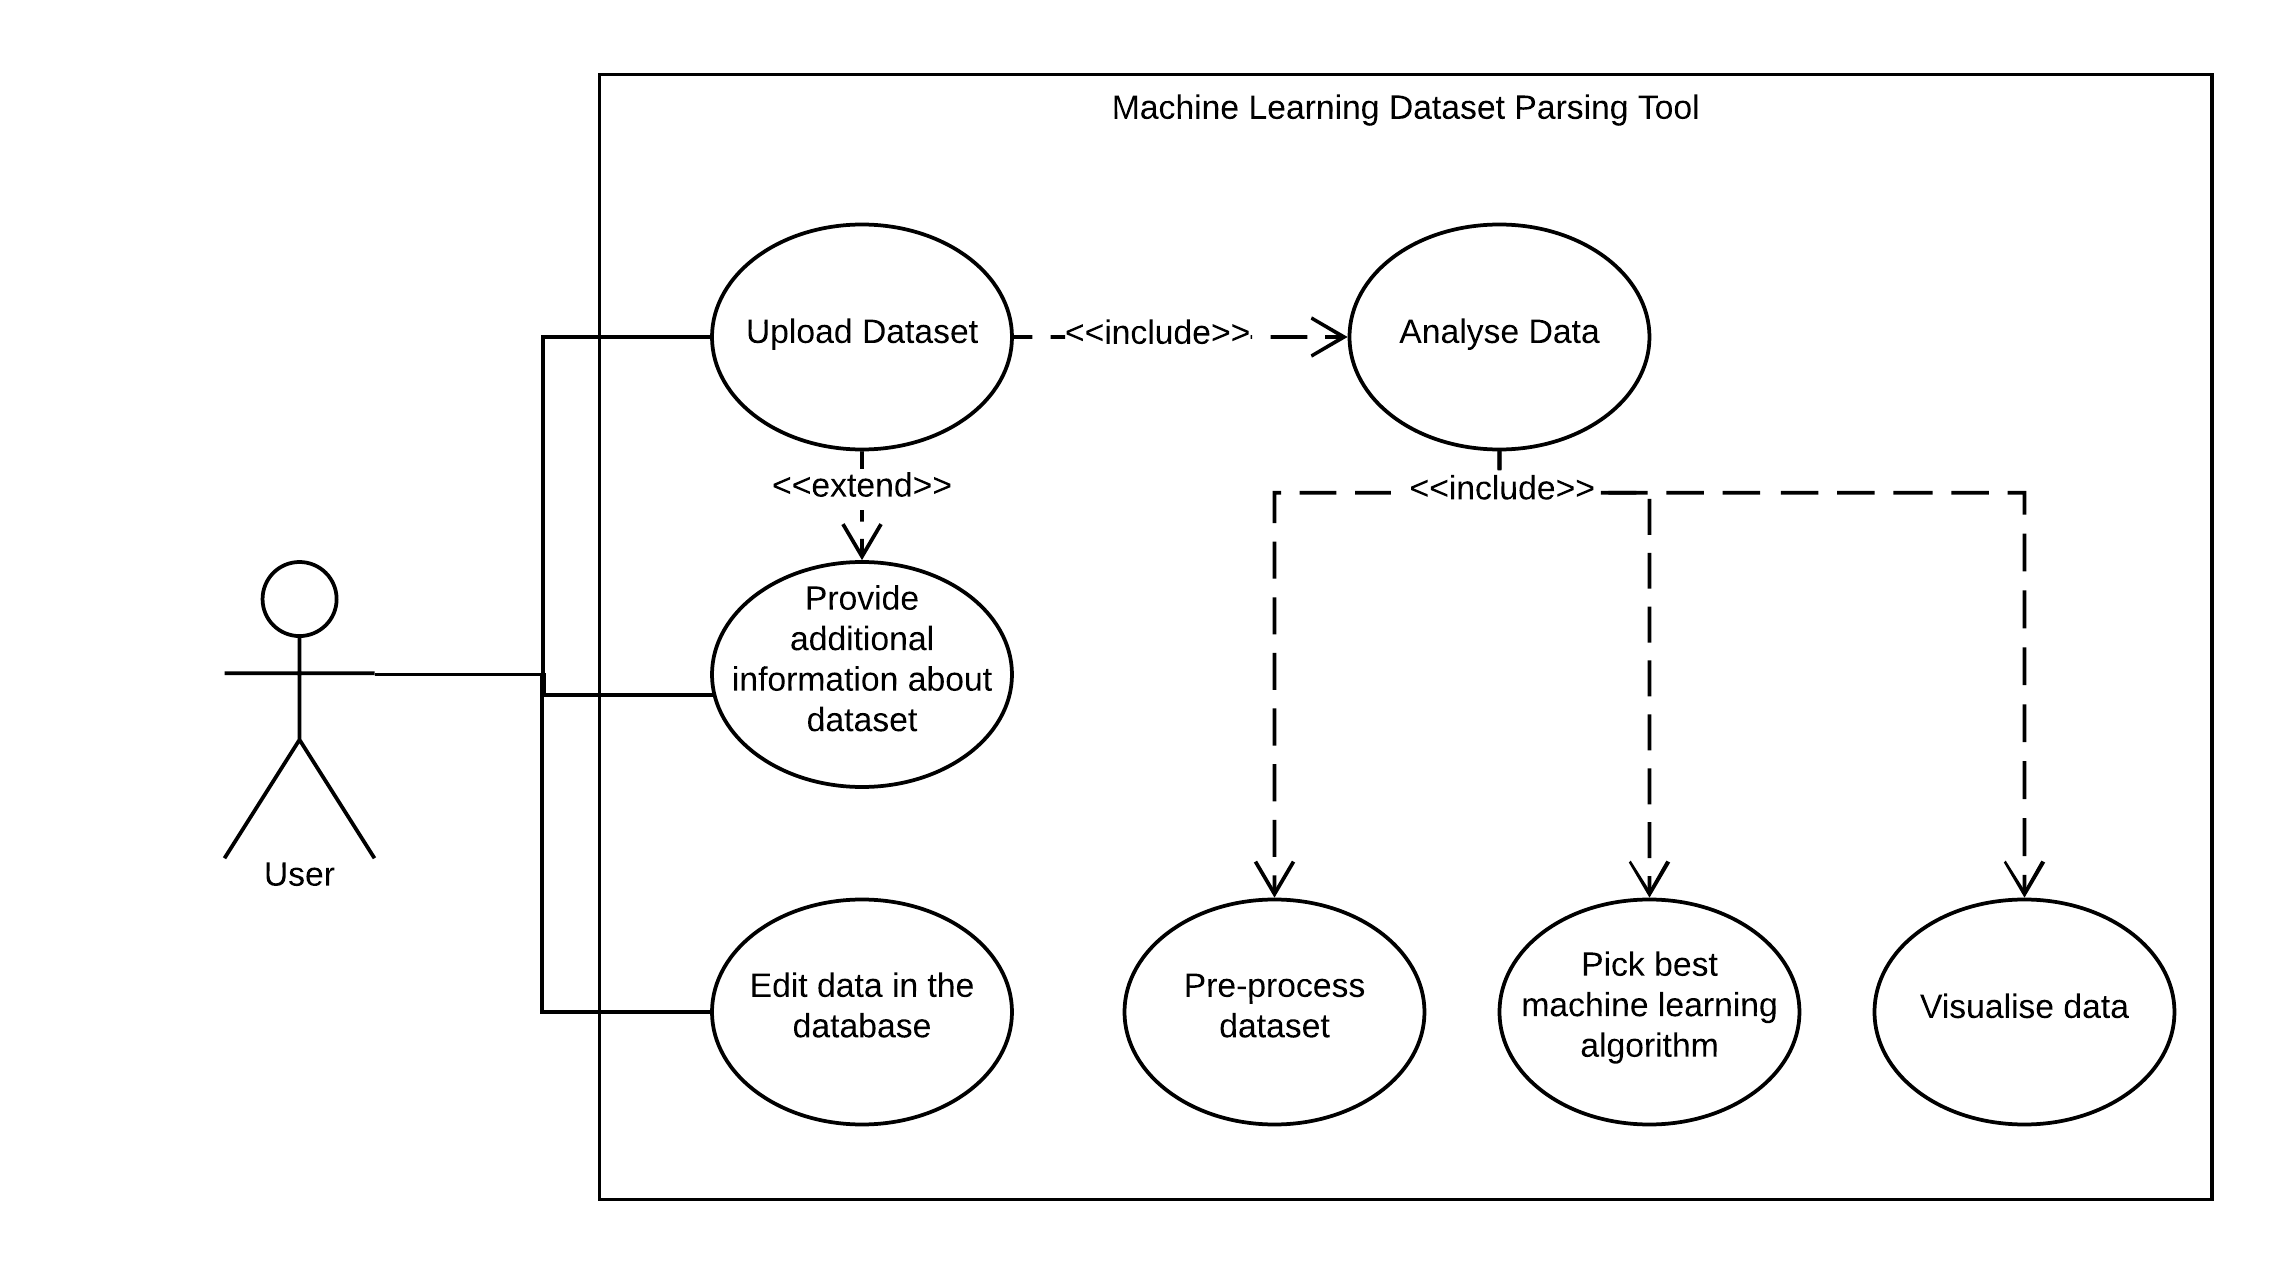
\includegraphics[width=\textwidth]{usecase}
  \caption{Simple use case diagram of the system}
  \label{usecase}
\end{figure}

The use case diagram clearly shows how the user will interact with the system.
Due to the nature of the system, much of its complexity is hidden from the user and therefore the user does not have many use cases.
Regardless, the use case diagram is an important part of the requirements gathering process as it makes it easier for the client to visualise their interactions with the system.

\section{Initial Design Ideas}
\subsection{Front End Design}
The user interface prototype is designed to accomodate the user requirements.
The home page will contain some information about the project, what it does, and how to use the tool.
The navigation bar, available on all pages of the site, contains links back to the home page, as well as to a page where users can see a list of datasets and analysis of a dataset.
From the home page, the user can choose to log in, see a list of the datasets in the system or upload a new dataset.
New users need an account to log in if they want to keep datasets private or delete datasets they have uploaded.
This feature will not be present in the first iteration of the project as it is not part of the core functionality, however the button will be in the front end, although not functional.

\begin{figure}[H]
  \centering
  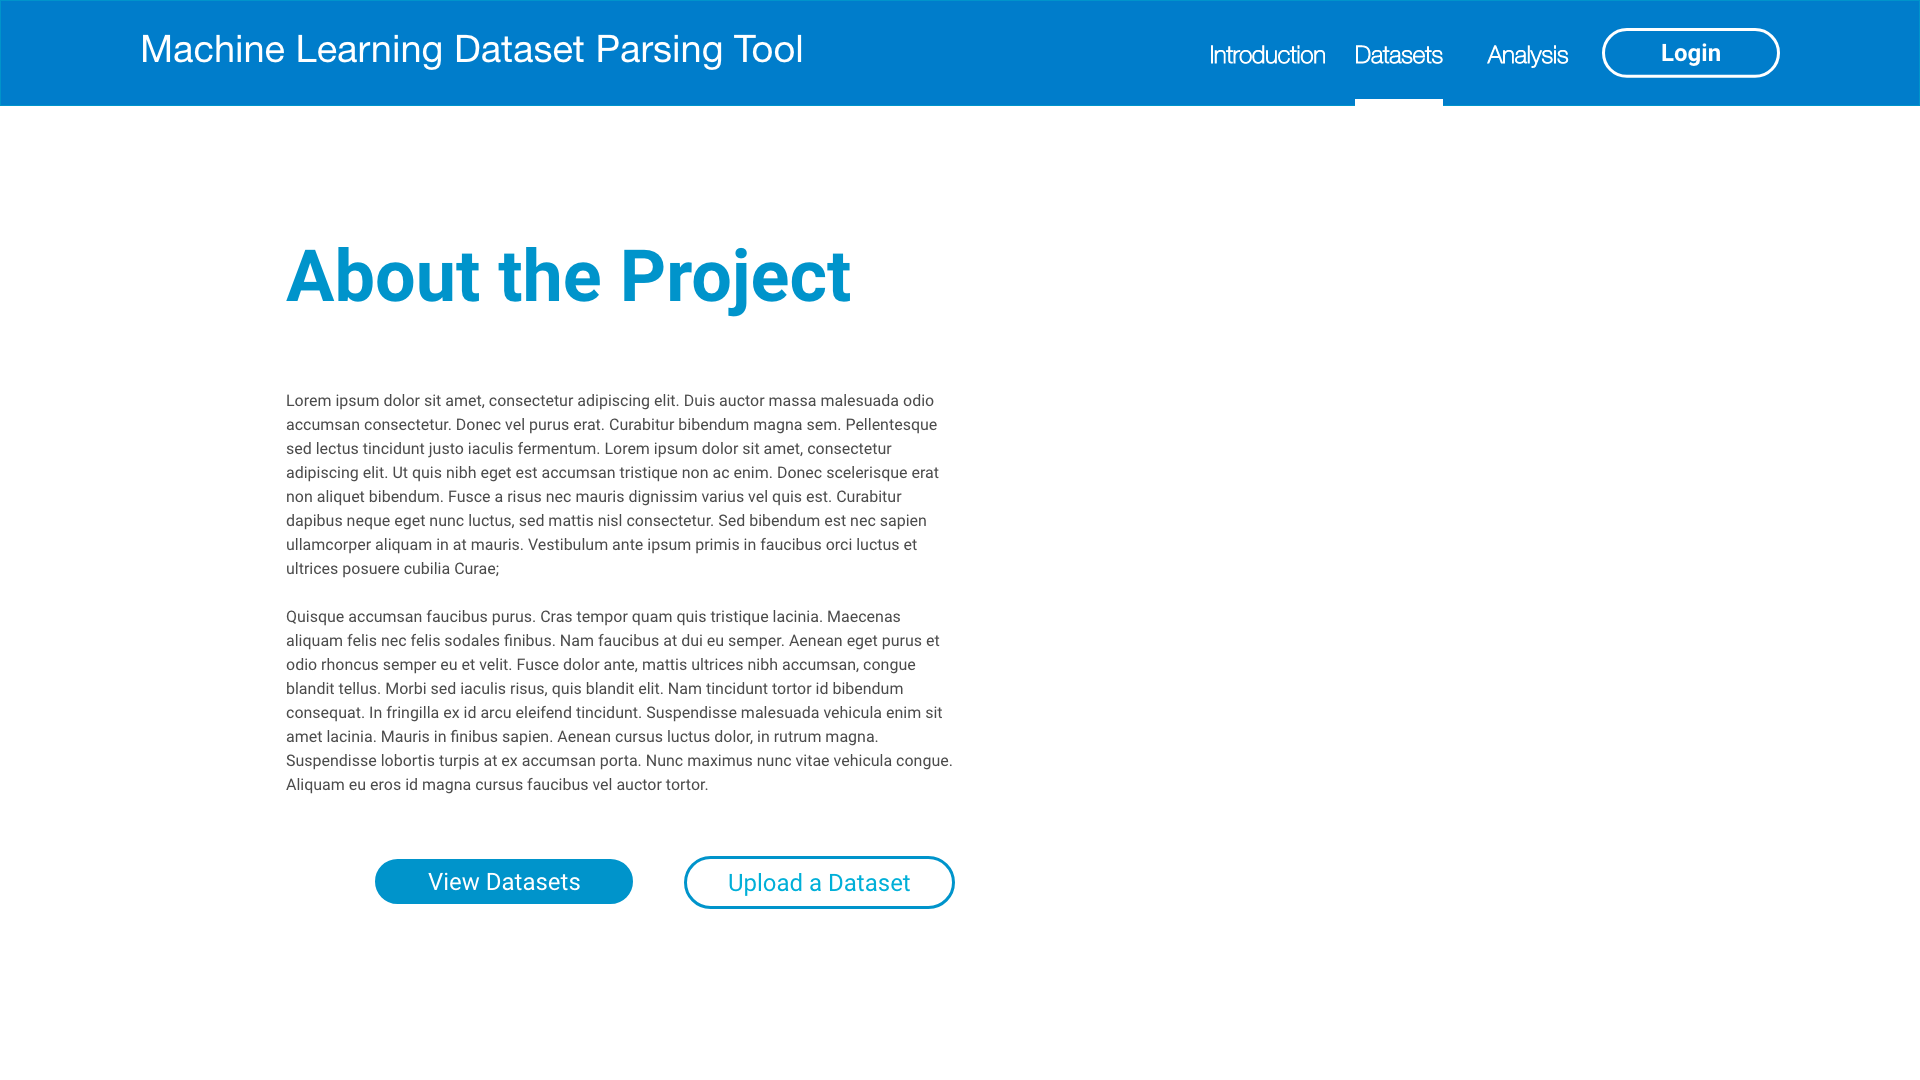
\includegraphics[width=\textwidth]{introduction_page}
  \caption{The Home Page of the system}
  \label{homepage}
\end{figure}

Clicking on the Datasets link takes the user to the Datasets page.
In the left part of the page, all files in the database list can be seen. Double clicking on a dataset takes the user to the visualisation page for that dataset.
From the Datasets page, the user may also choose to upload a new dataset for analysis.
There exists a search bar, clearly visible in the top right corner, where the user can search for datasets in the databse by name.

\begin{figure}[H]
  \centering
  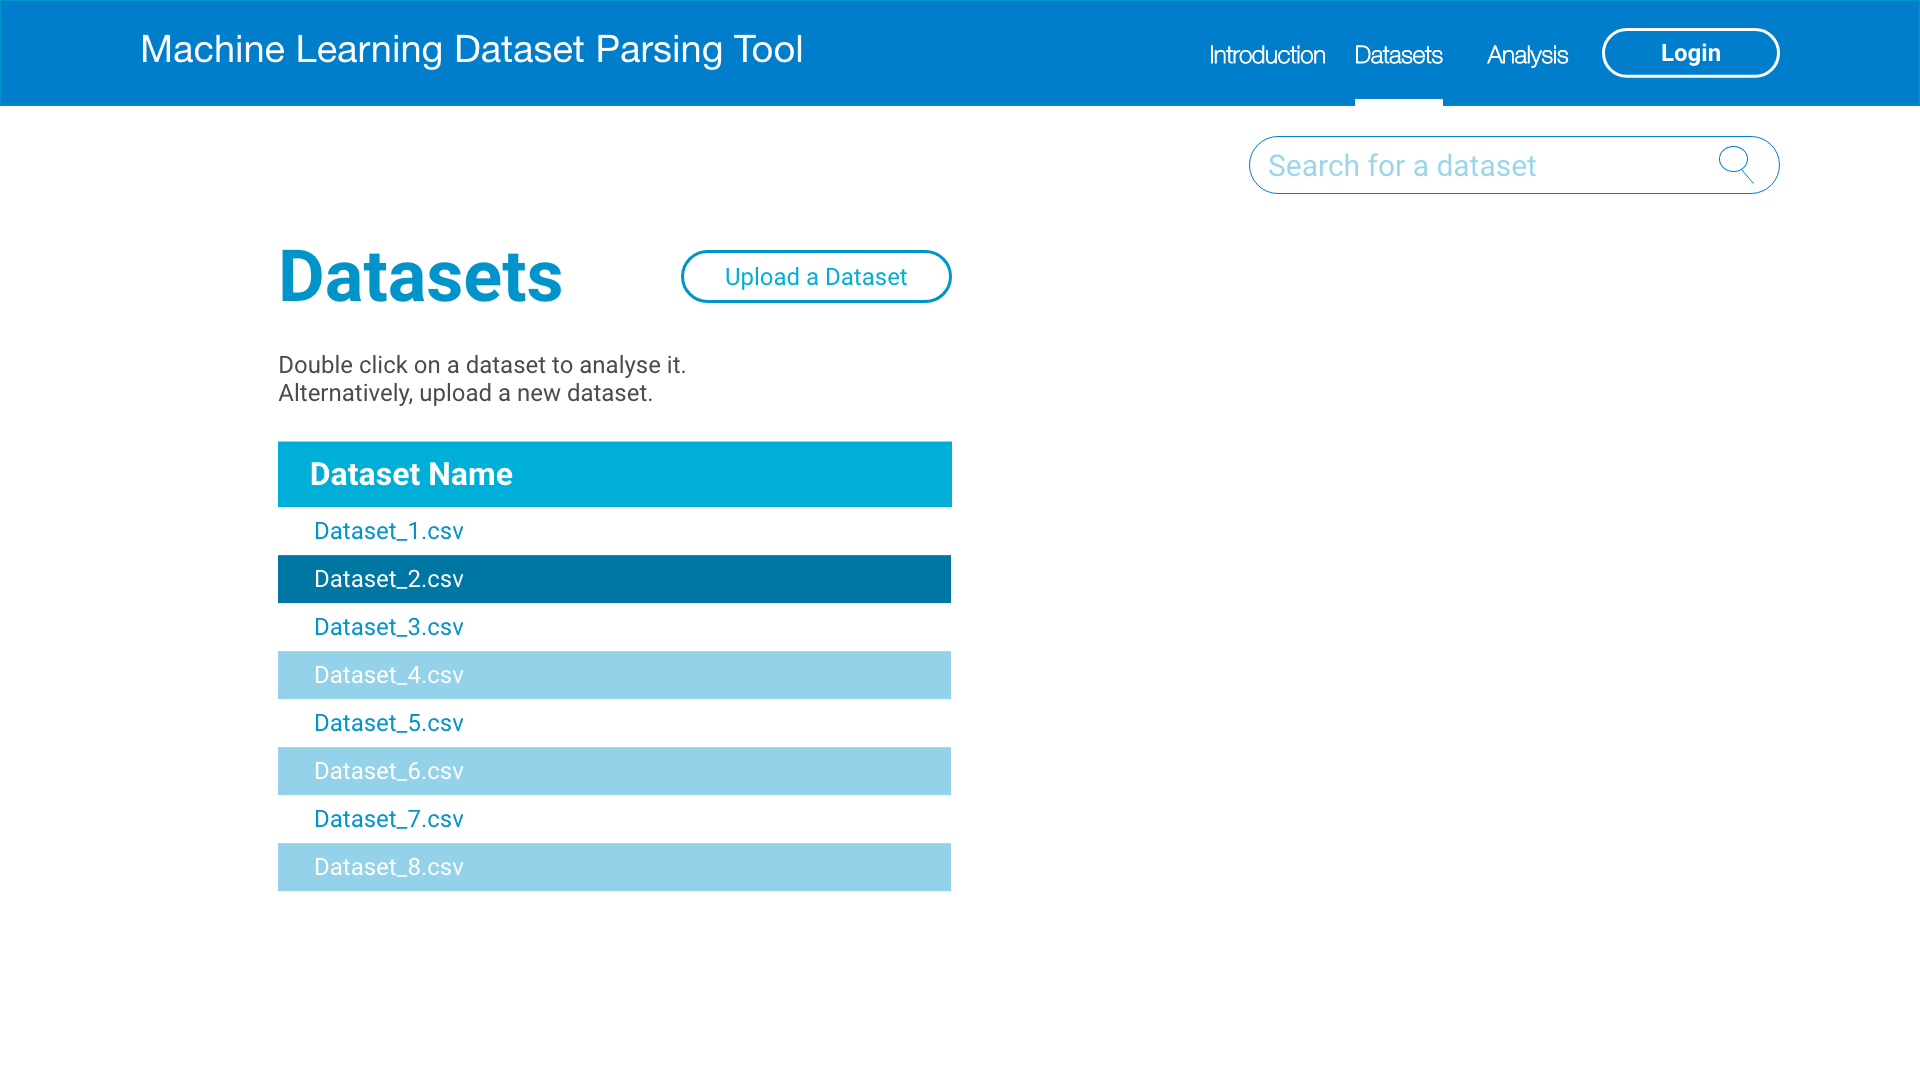
\includegraphics[width=\textwidth]{datasets_page}
  \caption{The Datasets Page of the system}
  \label{datasets_page}
\end{figure}

When a user double clicks on a dataset, they are taken to a page where the dataset is analysed.
The main function of the Analysis page for a dataset is to show the best machine learning algorithm for that dataset.
The dataset's name can clearly be seen at the top of the page.
More information about the dataset is available on the page, such as the features extracted by the data pre-processing routines outlined in section \ref{datarepresentation}.
Moreover, the user can see the decision tree and the route taken through the decision tree to get to the machine leanring algorithm that was chosen.
This is helpful for when the system is being used as a teaching aid, as it shows how the machine learnign algorithm was decided.
The user can also influence the decision made by changing the features that were extracted using the Edit button.
A download and delete button are also available, however the delete button will only be available to the user who uploaded the data set in futute iterations.
Clicking the download button will download the raw data, in CSV format (see section \ref{csvchoice}).
From the analysis page, the user can go to a page where the datasets are visualised.

\begin{figure}[H]
  \centering
  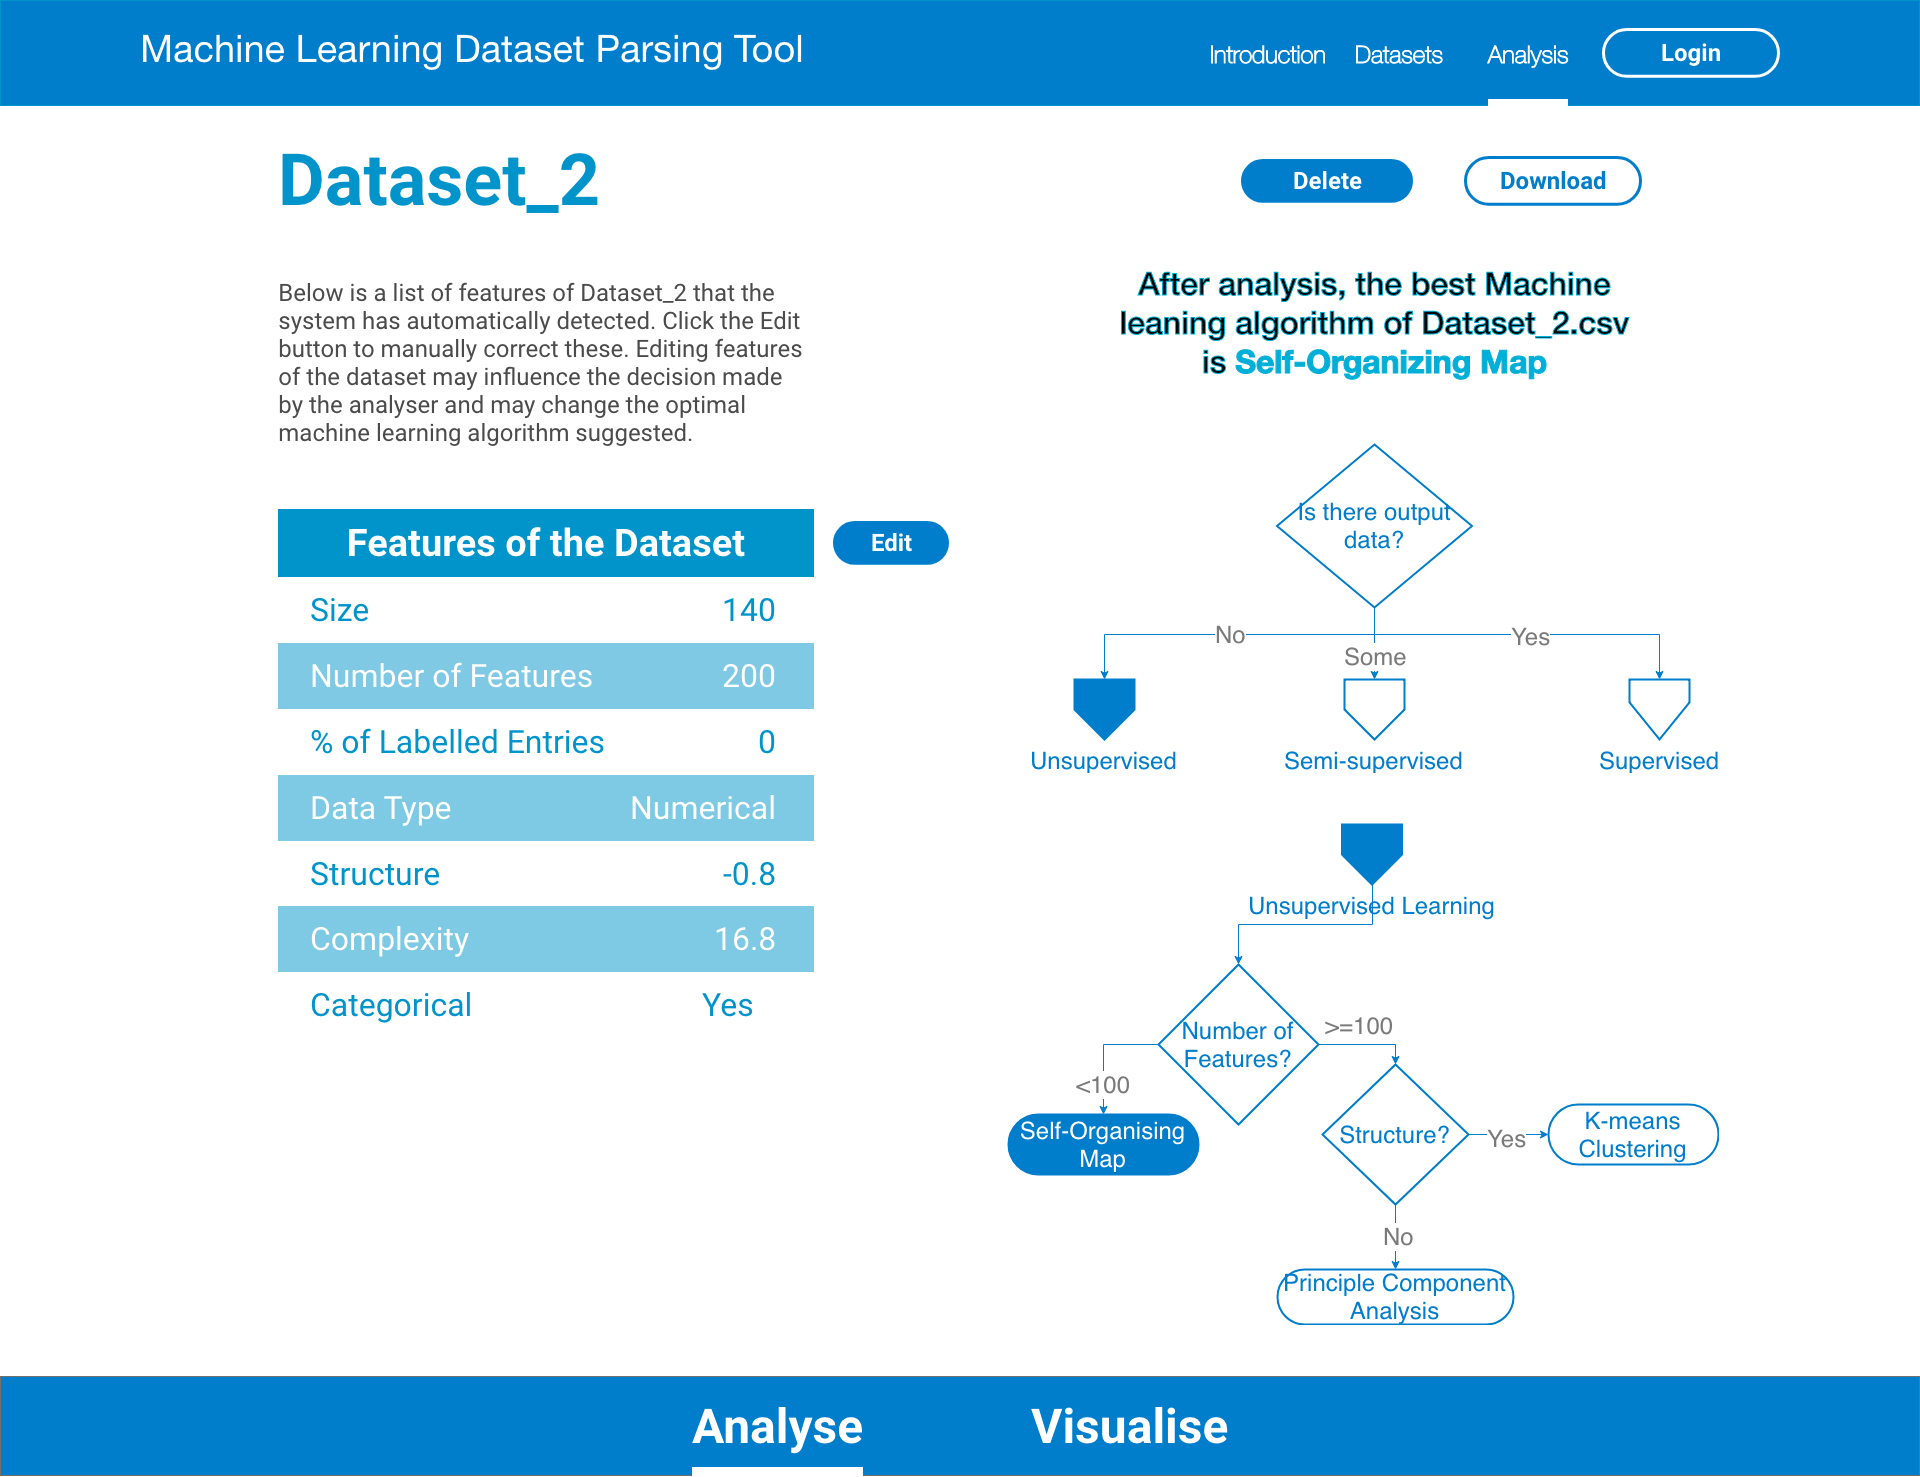
\includegraphics[width=\textwidth]{analysis_page}
  \caption{The Analysis Page of the system}
  \label{analysis_page}
\end{figure}

In the Visualisation page, the name of the dataset being visualised is shown at the top.
The user can choose different types of visualisation for the dataset, such as the raw tabular data, bar charts or scatter graphs.
The user can swap between these modes of visualisation, depending on the type of data that the dataset contains.
At the bottom of the visualisation page, the user can choose to show the analysis page for that dataset.
As data visualisation is not part of the core functionality, this feature will also not be present in the first iteration, but the group has accomodated for it in the design.

\begin{figure}[H]
  \centering
  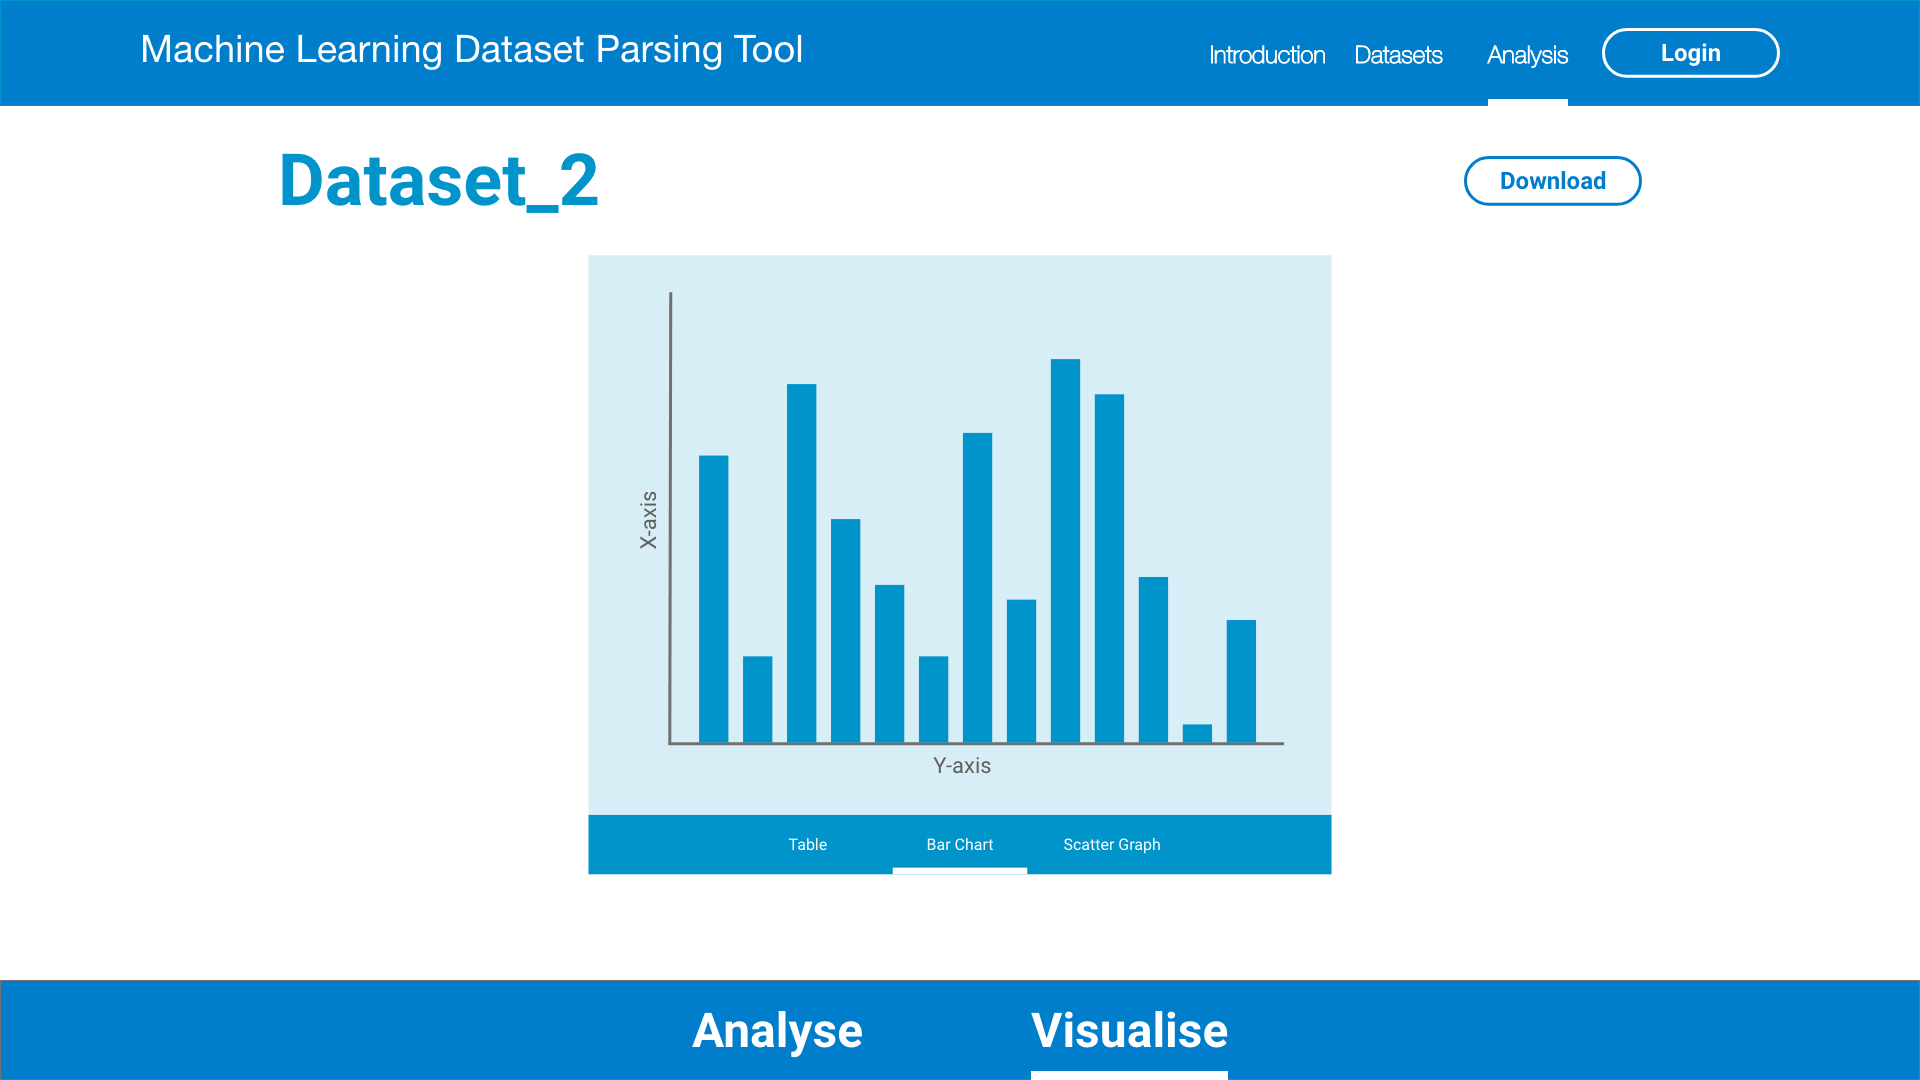
\includegraphics[width=\textwidth]{visualisation_page}
  \caption{The Visualisation Page of the system}
  \label{visualisation_page}
\end{figure}

\subsection{Picking the Machine Learning Approach} \label{pickingML}
The final goal of the project is to analyze datasets and automatically suggest the best machine learning tools by using our machine learning analyzer.
The analyzer will initially be composed of a Decision Tree, which will identify the best machine learning approach based on features of a given dataset.

The short-term goal is to classify dataset into three broad categories: Supervised Learning, Unsupervised Learning and Semi-supervised Learning according to whether there is output data in the dataset.
In order to provide a prototype to the client, the system will pick a random machine learning approah.
This will let the client have an idea of what a working system would function like.

The team decide to provide 17 potential machine learning tools:
% \setlength{\columnsep}{-2.1in}
\begin{multicols}{2}
\begin{itemize}
  \item Multiclass Neural Network
  \item Linear Regression
  \item Random Forest Regression
  \item Sum Regression
  \item Logistic Regression
  \item Neural Network
  \item Naive Bayesian Network
  \item Support Vector Machine
  \item Anti-learning
  \item Self-Organizing Map
  \item K-means Clustering
  \item Principle Component Analysis
  \item Forced Clustering
  \item Self-Training
  \item Deep Learning
  \item Recurrent Neural Network
  \item Time Delay Neural Network
  \item Feature Selection Principal Component Analysis
\end{itemize}
\end{multicols}

The most suitable tool will be suggested from this list of machine learning methods by using decision algorithm outlined below.

The website will display the selected most suitable machine learning tool for each dataset uploaded by client.
In the long term, the team hopes that the website will be able to analyze the dataset by using the best machine learning tool and visualize the output.
However, the team and client are both aware that given time constraints, it may not be possible to implement all 17 algorithms, and as such it was agreed with the client that although it would be useful to have, it is not part of the core functionality.

The decision algorithm will be used to determine which is the best analyzing algorithm for datasets.
First of all, the algorithm will determine whether the dataset is supervised; according to whether there is output data in the dataset, the dataset will be divided into three categories: Unsupervised Learning, Semi-supervised Learning and Supervised Learning, as can be seen in figure \ref{main-decision}.

\begin{figure}[H]
  \centering
  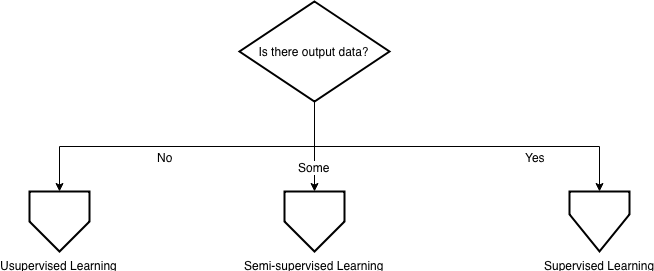
\includegraphics[width=\textwidth]{main-decision}
  \caption{Deciding the class of machine learning to use}
  \label{main-decision}
\end{figure}

If the dataset has no output data, it is classed as an Unsupervised Learning problem.
Within Unsupervised Learning, if there are lots of features in the dataset, suggest using a Self-Organizing Map to analyze. Otherwise judge whether the dataset have structure or not.
If they have structure, suggest K-means Clustering to analyze, otherwise suggest using Principal Component Analysis.
This deicion is modelled in figure \ref{unsupervised-decision}.

\begin{figure}[H]
  \centering
  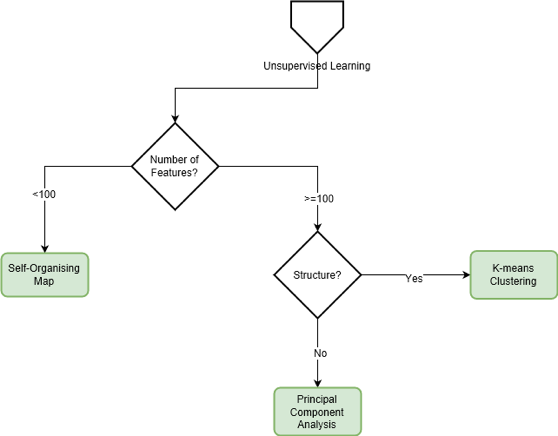
\includegraphics[width=\textwidth]{unsupervised-decision}
  \caption{Deciding which unsupervised learning technique to suggest}
  \label{unsupervised-decision}
\end{figure}


If the dataset is completely labelled with output data, divide it into Supervised Learning.
If the outputs are categories divide the dataset to Classification.
Otherwise if the outputs are continuous values, divide the dataset into Regression.

If the dataset is best modelled by classification, determine how many categories the dataset contains.
For a dataset with 3 or more categories, determine if the dataset is simple or not.
For small complex datasets, suggest Multiclass Neural Network or Random Forest Regression.
For simple large dataset, suggest using Multiclass Logistic Regression to analyze.
For datasets with less than 3 categories, determine whether the relations in the dataset are simple.
If the dataset has simple relations, suggest Logistic Regression. Otherwise determine how many features in the dataset.
If the dataset has less than 100 features, suggest Neural Network, otherwise suggest Naïve Bayesian Classifier or Support Vector Machine.
If, after modelling the data using a Naïve Bayesian Classifier or Support Vector Machine, the output is worse than guessing, suggest Anti-learning.

If the dataset is composed of values (regression), also determine the dataset simple or not. For a simple large dataset, suggest Linear Regression, conversely suggest Random Forest Regression and Sum Regression for a complex small dataset.
Figure \ref{supervised-decision} vizualises this set of decisions.

\begin{figure}[H]
  \centering
  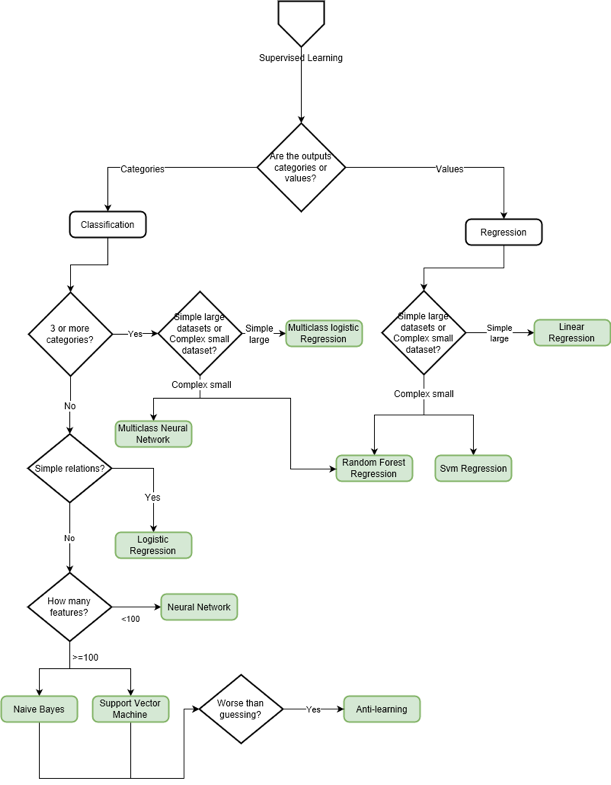
\includegraphics[width=\textwidth]{supervised-decision}
  \caption{Deciding which supervised learning technique to suggest}
  \label{supervised-decision}
\end{figure}


Semi-Supervised Learning is a class of machine learning tasks and techniques that also makes use of unlabeled data for training – typically a small amount of labeled data with a large amount of unlabeled data.
If only 33\% or fewer of the entries in the dataset are labelled, suggest Self-Training.
Otherwise suggest using self-Training to analyze.
The semi-supervised decision is shown in figure \ref{semisupervised-decision}.

\begin{figure}[H]
  \centering
  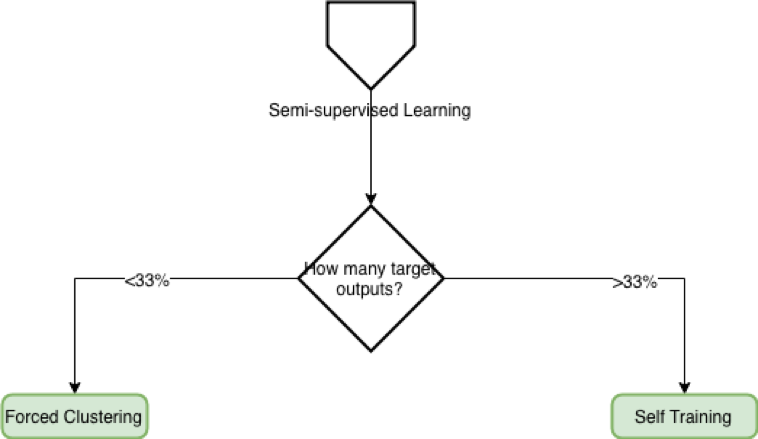
\includegraphics[width=\textwidth]{semi-supervised}
  \caption{Deciding which semi-supervised learning technique to suggest}
  \label{semisupervised-decision}
\end{figure}

\subsection{Data Representation\label{datarepresentation}}
Section \ref{csvchoice} outlines the allowed file types in the system.
However, data preprocessing is needed in order to choose the most suitable machine learning algorithm, as it is required that information about the dataset (such as whether or not there are missing labels, its complexity, whether the output is categorical or not) is available for the decision based algorithm.
As such, before data are uploaded to the database, a pre-processing script extracts features and stores them, alongside the data, in an Object.
The object has the following fields holding the specified data types:

\begin{alltt}
  dataset: \{
    name: string,
    headings: list of strings,
    number-of-features: integer,
    values: matrix of values,
    missing-values: list of coordinates,
    original-values\footnotemark: matrix of values,\footnotetext{This field will only exist if there are missing values, where the missing values are imputed in the "values" field, but a copy of the original values is kept in the "original-values" field}
    anomalies: list of coordinates,
    labels: list of strings,
    missing-labels: list of integers,
    data-type: string,
    size: integer,
    labels-ratio: number \((0 \leq x \leq 1)\),
    is-categorical: true / false,
    categories\footnotemark: list of strings, \footnotetext{This will only exist if the data is deemed categorical}
    complexity: number,
    structure: number \((-1 \leq x \leq 1)\),
    relations: list of features
  \}
\end{alltt}

A short explanation of each field is provided below where the name-value pair does not make it obvious:
\begin{itemize}
  \item \verb|values, original-values|: the original data (and potentially imputed data) from the input CSV file, stored as a matrix
  \item \verb|missing-values, anomalies|: the coordinate into the \verb|values| or \\\verb|original-values| matrices where missing or anomalous values can be found
  \item \verb|labels-ratio|: the total number of rows of data divided by the number of missing labels
  \item \verb|complexity|: a numerical score of the complexity of the dataset, based on the average bias-corrected variance of each column
  \item \verb|structure|: a numerical score of the average correlation coefficient of each column
  \item \verb|relations|: list of columns that could be related, determined by pairs of columns with high correlation coefficients
\end{itemize}

\section{Key Implementation Decisions}
\subsection{Programming Languages}
When deciding which languages would be most suitable for the project, a few aspects that were considered were functionality, familiarity  and convenience.
Functionality was the main concern, given that the system is a web-based project.
Therefore, the group needed to choose a language that could interface easily with a web application.
Familiarity made this decision more difficult, as only one group member was familiar with JavaScript, which is the main language used on the web.
As such, the group had to pick a range of languages that accomodated both the functionality needed as well as the experience level of the group members.
Convenience therefore became an issue, as all group members had to ensure that code in one language could easily interface with code from another language.

Apart from HTML and CSS, both of which are essential to any web application, a few languages discussed are listed below.
\begin{enumerate}
  \item \textbf{JavaScript} is a web scripting language.
  JavaScript enables interactive web pages and thus is an essential part of web applications.
  It is a dynamic\cite{js_datatypes} weakly typed language.
  Its primary purpose is to provide interactivity and have programatic control over elements on a web-page \cite{jsWhatIsJavascript}.
  As a simple web-based project, most functionality needed at this stage can be implement by JavaScript.
  JavaScript also has an extensive collection of libraries, as well as a server-side runtime environment (Node.js \cite{nodejs}), which makes it suitable to use in the back-end of a web application.
  As discussed in section \ref{dbdesign}, a NoSQL MongoDB database was chosen, and Node.js contains a library (Mongoose \cite{mongoose}) which makes implementing the database easy with a Node.js framework.

  \item \textbf{PHP} is a scripting language tailored for the web \cite{php}.
  PHP code can be integrated into Java, C and Perl and can be embedded into HTML code.
  It is weakly typed\cite{php_datatypes} and has a high developing efficiency to complete an activity web page.
  It is easy to learn, the source code can be found easily on webpages.
  It also can connect MongoDB.
  It could be used to develop server-side functionality of the project.

  \item \textbf{Java} is the language the group is most familiar with.
  There exist good Integrated Development Environments (IDEs) such as Eclipse and IntelliJ which we have all used before. It has a security structure and easy to debug.
  But the code would be more verbose than other languages and it is more difficult to make connection with HTML webpage.
  In other words, Java is suitable for some big projects that need precise design.
  Java code could be implemented on webpages with Java Server Pages \cite{jsp}, but this would add a lot of uneccessary overhead.

  \item \textbf{Python} is a language with simple structure.
  It is easy to master and can implement functions in fewer lines code.
  The shortcoming is that it is unfamiliar to the group, and so choosing it might cause unpredictable problems such as environment building which lead to the work goes slowly.
  Python code can be implemented on webpages via the Common Gateway Interface (CGI) \cite{python_web}.
\end{enumerate}

Due to both convenience and functionality, as described above, the group decided the main language used to implement the system would be JavaScript.
JavaScript can also run both in the browser client-side, or in the server, meaning that the system can be more universally accessible on all devices with a web browser.
It should be noted that due to limitation in its ability to perform machine learning algorithms on large datasets (a task that languages such as Python and R are very well established in), the group may have to incorporate other languages.
However, JavaScript proves both convenient and capable enough for the first iterations of the system.
Due to its low learning curve and past experience in the group, it will not be too difficult for everyone who needs to use it to learn enough to produce a capable system.

\subsection{Design Pattern}
As outlined in section \ref{work_division}, the group has divided the workload into three parts: Machine Learning, Database Implementation and Front End Development.
These three elements of the system loosely fit the description of the \textit{Model-View-Controller} (MVC) design pattern \cite{google_mvc}.
This allows for better code organisation and maintainability \cite{google_mvc} by seperating responsibilities within the codebase.
The three key components of the MVC design pattern are outlined below:
\begin{itemize}
  \item \textbf{Model}:
  This is where the data of the system is stored.
  The Model has no access to the View or the Controller, and is only responsible for storing the data.
  This is essentialy the Database of the project.
  \item \textbf{View}:
  This is how the user inteacts with the system, and how the system presents data to the user: the Front-End.
  Although the user interacts with the View, the View has no responsibilities apart from to display the data in the Model.
  \item \textbf{Controller}:
  The Controller acts as the bridge between the Model and the View; it updates the View when changes happen to the Model, and updates the Model when the user interacts with the View.
  This is the Machine Learning section of the group's work division.
  The controller is responsible for all logic in the system.
\end{itemize}

Although the MVC design pattern is being employed in this project, the project need not adhere strictly to it.
Its ideas and philosophies are useful in that they allow seperation of concerns thus creating more maintainable code, however the project does not lend itself well to a strict implementation of the pattern given that its main concern is data processing.

\subsection{Database Design\label{dbdesign}}
\subsubsection{NoSQL vs SQL}
Heterogenous big data benefits from NoSQL for a few reasons.
Firstly, there is no predefined schema that the data has to conform to, which is useful for our application as it will have to save data from a multitude of different data sources in the same data store.
It is not possible to index all the data efficiently beforehand, and therefore a large schema that all datasets will conform to cannot be defined.
Even if this was easily possible, a large schema would waste a lot of space, as most datasets would only use a small subset of the schema.
This would also make searching the database very inefficient, as it would be resource inefficient to have to search through potentially hundreds of unused fields.

Removing schemas also makes the database faster to query \cite{sqlvsnosql}.
Because each dataset is stored in one document rather than spread across multiple tables, the program knows exactly where to look for the data set rather than having to search through multiple tables.
This helps when having to search through a lot of datasets to find the data set of interest.

\subsubsection{Lack of Relations Between Datasets}
The data sets that our program will use contain almost no relations.
As such, using a relational database would waste a lot of the functionality associated with relations, and cause a lot of uneccessary overhead.
Instead, a non-relational database will just store data sets independently of each other.
Querying the database will simply involve returning a JSON object, with no links to other data sets.

\subsection{Accepted File Types in the System\label{csvchoice}}

When studying Weka, the team found that there are many file types that machine learning tools could use, for instance Arff data files, CSV data files, XRFF data files, amongst others.
After some research into the UCI Machine Learning Repository \cite{uci}, the team decided to use CSV data files to store datasets into the database and to be used by the machine learning tools.
This decision was also agreed upon by the client, who stated that CSV file types would suffice for the core functionality of the system.
Other file types were welcomed, but not required.

CSV files were chosen as they make it convenient for the team to transform the .data files and .name files found on the UCI repository into a single file.
CSV files are also easy to store in the NoSQL database.
Knowing the format of the data is useful for data pre-processing and analysing.

\section{Problems Encountered}

\subsection{Time and Project Management}
Although in theory our Agile time planning workflow outlined in section \ref{timeplanning} was solid and fitted the needs of both the client and team, in practice the team found some flaws.
Firstly, due to there being no planned strict deadlines apart from those imposed in the GRP Handbook, deliverables were not always completed on time.
Although things would get planned and discussed in the meetings, group members often forgot or did not check the minutes of the meetings to find what they needed to do.
This would have not been the case had there been a formalised time plan set out near the start of the project.
Moreover, even though the team set out some soft deadlines, for example having a working first version of the application by the report deadline, there was no real incentive to actually acomplish this goal and so it was not completed.
Had the team set out a Gantt chart, for example, everyone would have deadlines to work towards and the incentive of having other team members rely on their part to be done would have been made clearer.

Moreover, the Kanban board that was set up was only used for the first few weeks of the project.
After that, most tasks that needed to be done were discussed through the meetings and on instant messaging, and while that did work, there was no centralised place where people could remind themselves of what needed to be done.

\subsection{Visualising the Output}
A few problems arose when deciding how to visualise the output of the data processing.
Firstly, choosing a suitable graph for each data set will be very difficult, given the nature of a data set cannot be known.
As such, a general form of visualisation has to be devised.

Moreover, due to the requirement that the system be used for a teaching aid, all visual indication of any analysis the system conducted had to be both educational and clear.
A textual analysis may have been educational, but not very clear, and as such the team decided to visualise the decision tree in the output.
However, visualising the tree proves difficult, as a technique for dynamically generating the tree must be devised.

\subsection{Programming Language Inexperience}
Since it was decided that Javascript would be the most convenient language to use for a web-based application, it became obvious that some members of the group would have to first learn the language.
Although it is a relatively easy language to learn, Javascript has enough complexity to make tasks such as implementing the decision tree quite challenging for beginners.
However, the group feels Javascript removes enough overhead when connecting the front and back ends to make it worth learning.

\subsection{Testing}
Before starting initial implementations, the group did not discuss a testing formalised plan.
This meant all group members had to informally test their own code by themselves, and even then no documentation was produced on the progress of the testing.
Test-driven development should be incorporated into the workflow of the team for the rest of the development cycle so as to ensure that testing is happening consistently.

However, due to the nature of the application, testing proves quite challenging.
A lot of the functionality of the system has to be mocked when unit testing as it is designed to work on larger datasets, which would take too long to test with in an efficient workflow.
Moreover, a lot of the units in the system are designed to work together, so testing them independently is difficult.
Maintaining a functional programming style as much as possible, especially when pre-processing datasets, increases testability as the functions are pure and provide predictable outputs.

\section{Time Planning and Project Management}
\subsection{Time Planning\label{timeplanning}}
For time planning, the team never formulated a rigid time plan like a Gantt chart, although this was discussed.
The idea behind not having a rigid time plan was that it would not be adhered to given other responsibilities the team has, potential changes to requirements and underestimation of the time needed to perform a task.
Instead, the team's time planning was dictated primarily through the weekly formal and informal meetings, where deliverables were agreed on with the supervisor on a weekly basis.
This allowed the team to have a more agile workflow by respecting the Agile Manifesto's `Responding to change over following a plan' and `Individuals and interactions over processes and tools' values \cite{agilemanifesto}.
Communication was a key component of this workflow, as the team had to regularly discuss and show progress made.
It also meant that the team was consistently and incrementally working on the project, as opposed to leaving tasks unfinished for long periods of time.

Regardless of not having a rigid time plan, the team set out some soft deadlines for major deliverables of the project.
This soft time plan is outlined below.

\begin{enumerate}
  \item \textbf{2018/12/14}: The report deadline. It was planned that the initial prototype would be finished by this date.
  \item \textbf{2018/02/18}: It was planned that by the start of the second term, the prototype would be further developed into a working first version.
  \item \textbf{2018/03/18}: The system will be able to fully visualise a given dataset. The decision making algorithm would be fully implemented and refined.
  \item \textbf{2018/04/11}: Final report deadline. The system will be complete and the final report written.
\end{enumerate}

\subsection{Project Management}
The team decided to use Kanban as its main form of project management. The Kanban board is hosted on Trello.com \cite{trello}.
Scrum was discussed as an alternative approach, but Kanban was chosen for some reasons outlined below:

\begin{itemize}
\item Teams using Kanban can cope with mutable requirements flexibly. Teamwork will continue with changing project environment.
\item Formal and informal meetings can be held as frequently as needed and agile working process can be pushed favorably by team communication.
\item Due to the main process of the project having been decided, Kanban is a good system as it allows us to vizualise every stage of work and everyone’s processing.
\item For a team with less development experience, it is difficult to deliver an executable program in a short time. Scrum would be difficult to practice because of its demand on techniques and experience.
\item Scrum need to stipulate working time for every iteration, which is difficult for teams with less development experience. Kanban only displays stage missions but not time limits.
\item Scrum needs to declare a Product Owner, Scrum manager and Team which might cause confusion in an inexperienced team. Kanban can make team members focus on their work and research.
\end{itemize}

After agreeing that Kanban would be more suitable to our team's needs, a Kanban board was created on Trello. Trello was chosen as it makes collaboration a lot easier.
Being a web based tool, it made it easy for us to manage our workflow from all of our devices, as well as accomodating remote work and management.
It also accomodates team collaboration as it allows people to join the Trello board, which was an essential feature the team needed in order to be able to manage its work collaboratively.

\subsection{Division of Work\label{work_division}}
Rather than everyone playing a role in every aspect of the project, it was decided it would be easier to divide the work into three distinct subgroups.
The project was divided into three main sections: \textit{Front-End Development}, \textit{Machine Learning} and \textit{Data Pre-processing and Database Development}.
It was decided that Hao and Xinyang would be responsible for Front-End Development, Boyan and Xinjie for Machine Learning and Marios for the Data Processing and Database.
The division was made based on both past experience with technologies needed for that area, as well as personal preference.
As such, there was no conflict in deciding who would be responsible for what area.

Dividing the project in this fashion allowed the team to be able to divide workload more efficiently, as any task could be categorised into one of the three areas of the project and assign the task to the correct person(s).

Following this division of labour, it was decided that the Kanban board would be better organised if there was a list for each section.
Therefore, three lists ("To Do", "Doing" and "Done") were created for each are of the project, as well as one set of lists for "Other" tasks that had to be done (for example, adding a section to the report, drawing diagrams).
This project management workflow kept everything atomic, where everyone was only responsible for a small subset of tasks.
It also kept people focused, as everyone could find the correct list for their section and pick up "To Do" tasks that correspond to their section of the project.

\pagebreak
\printbibliography

\end{document}
